% RCR-YOLO Paper LaTeX Source (English Version)
% Compiler: pdfLaTeX (IEEEtran default Times setup)
% Template: IEEE Transactions

\documentclass[journal]{IEEEtran}
\DeclareFontShape{OT1}{ptm}{bx}{n}{<->ssub*ptm/b/n}{}
\DeclareFontShape{OT1}{ptm}{bx}{it}{<->ssub*ptm/b/it}{}
\usepackage[utf8]{inputenc}
\DeclareUnicodeCharacter{00B1}{\ensuremath{\pm}}
\DeclareUnicodeCharacter{00D7}{\ensuremath{\times}}
\DeclareUnicodeCharacter{00B2}{\textsuperscript{2}}
\DeclareUnicodeCharacter{2014}{---}
\DeclareUnicodeCharacter{2013}{--}

% Basic packages
\usepackage{cite}
\usepackage{amsmath,amssymb,amsfonts}
\usepackage{algorithmic}
\usepackage{graphicx}
\usepackage{textcomp}
\usepackage{xcolor}
\usepackage{booktabs}
\usepackage{microtype}

% Hyperlinks
\usepackage{hyperref}
\hypersetup{
    colorlinks=true,
    linkcolor=blue,
    filecolor=magenta,
    urlcolor=cyan,
}

% Document information
\title{RCR-YOLO: Robust Context-aware Region Detection for Indoor Object Detection}

\author{Author Name (To be filled)}

\begin{document}

\maketitle

% ==================== Abstract ====================
\begin{abstract}
Indoor object detection faces challenges from small scales, occlusion, and crowding that degrade general detector performance. We propose RCR-YOLO, a robust detection method based on YOLO11n with three complementary modules. ORB-In provides training-time auxiliary supervision through object region and boundary reconstruction, enhancing small object feature learning with zero inference cost. MRFE employs a multi-receptive field mechanism to improve multi-scale representations via parallel dilated convolutions and dynamic weighting. LCRBase integrates lightweight scene-level context through multi-scale pooling, simplifying full context reasoning for stable single-stage integration. Systematic ablation studies on COCO-indoor validate the contribution and synergy of each component. Our method achieves 0.3433 mAP50-95 (+3.7\% vs baseline) and 0.3343 Hard AP50-95 (+3.8\%), with consistent improvements across small objects, occlusion, and crowded scenes. Three-seed validation demonstrates superior stability (AP50-95 std ±0.0005 vs baseline ±0.0012). The deployed model requires 3.17M parameters with 10.36ms latency on RTX 4090, maintaining real-time performance (~96 FPS). Results demonstrate effective adaptation of two-stage context mechanisms to single-stage detection frameworks for indoor environments.
\end{abstract}

\begin{IEEEkeywords}
Object detection, Indoor environment, Multi-receptive field, Context reasoning, YOLO, Service robots
\end{IEEEkeywords}

% ==================== Section I: Introduction ====================
\section{Introduction}
\label{sec:introduction}

\subsection{Motivation and Background}

Indoor service robots are increasingly deployed in household assistance, healthcare, smart warehousing, and elderly care facilities \cite{service_robot1,service_robot2}. Reliable object detection serves as a fundamental capability for autonomous navigation, human-robot interaction, and task execution. However, indoor environments present unique challenges that distinguish them significantly from the outdoor or general detection scenarios commonly addressed in existing literature.

In indoor scenes, the object scale distribution is biased toward small desktop items (cups, remote controls, phones, keyboards, etc.), which occupy only a few pixels in feature maps and are easily overwhelmed by background clutter. Occlusion is ubiquitous — mutual occlusion among furniture, human bodies, and objects leads to partially visible targets and blurred boundaries, requiring robust spatial reasoning to infer complete object shapes. Scene crowding is another prevalent characteristic — bookshelves, desktops, and kitchen countertops often exhibit densely arranged objects with heavily overlapping bounding boxes, making effective utilization of rich contextual information difficult. These challenges intertwine in typical service robot working environments, posing severe tests for detection systems.

Existing general-purpose detectors such as the YOLO series \cite{redmon2016yolo,bochkovskiy2020yolov4,ultralytics2023yolov8} and R-CNN family \cite{girshick2014rcnn,ren2015faster} have achieved impressive results on large-scale datasets (such as MS COCO \cite{lin2014microsoft}). However, these methods are optimized for balanced performance across all COCO categories and exhibit degraded performance in indoor-specific scenarios. Limitations include: (1) insufficient supervision for low-level feature learning — standard detection losses only impose constraints at positive anchor locations, providing weak guidance for spatial distribution and contour learning of small objects; (2) limited multi-scale representation capability — convolutions with fixed receptive fields struggle to adapt to extreme scale variations from a few pixels to hundreds of pixels; (3) underutilization of contextual information — general detectors lack explicit context reasoning mechanisms for indoor occlusion and crowded scenes. Specialized designs for indoor scenarios remain insufficient.

Inspired by the success of reconstruction tasks in representation learning, the effectiveness of multi-receptive field mechanisms in multi-scale detection, and the potential of context reasoning in challenging scenarios, we propose RCR-YOLO, a robust context-aware detection method tailored for indoor environments. Building on the lightweight YOLO11n architecture, we design three complementary modules: ORB-In provides auxiliary supervision through training-time object region and boundary reconstruction, enhancing low-level feature learning for small objects with zero inference cost; MRFE employs a multi-receptive field mechanism to improve multi-scale representations via parallel dilated convolutions and dynamic weighting; LCRBase integrates lightweight scene-level context through multi-scale pooling, simplifying full context reasoning for stable single-stage integration. Systematic ablation studies on the COCO-indoor dataset validate the independent contribution and synergistic effects of each component, while three-seed validation demonstrates the stability and reliability of our method.

\subsection{Main Contributions}

The main contributions of this paper are summarized as follows:

\begin{enumerate}
    \item \textbf{RCR-YOLO Architecture}: We propose a detection method tailored for indoor environments, where three complementary modules (ORB-In, MRFE, LCRBase) synergistically enhance YOLO11n, providing specialized designs for indoor challenges including small objects, occlusion, and crowding.

    \item \textbf{Train-Inference Asymmetric Design}: The ORB-In module provides object region and boundary reconstruction supervision during training to enhance low-level feature learning, while being completely bypassed during inference to achieve zero inference cost, balancing performance improvement with real-time requirements.

    \item \textbf{Single-Stage Context Reasoning Adaptation}: LCRBase simplifies the difficulty gating and region aggregation mechanisms of full LCR, retaining only scene-level context enhancement, resolving the instability issue of two-stage context reasoning methods in single-stage detectors (three-seed validation shows 5× variance reduction).

    \item \textbf{Systematic Evaluation and Validation}: We conduct 10-configuration ablation experiments on the COCO-indoor dataset, perform three-seed validation on key models to assess stability, evaluate challenging scene performance with the Hard v2 protocol, and provide qualitative visualizations showcasing practical improvements.

    \item \textbf{Practical Performance}: The ab4-rcr-fb configuration achieves 0.3433 mAP50-95 (+3.7\% vs baseline) and 0.3343 Hard AP50-95 (+3.8\%), with consistent improvements across small objects, occlusion, and crowded scenes, while maintaining real-time performance (~96 FPS, 3.17M parameters, 10.36ms latency).
\end{enumerate}

\subsection{Paper Organization}

The remainder of this paper is organized as follows: Section~\ref{sec:related_work} reviews related work, including general object detection, indoor detection methods, feature enhancement techniques, and context modeling. Section~\ref{sec:methodology} details the RCR-YOLO architecture, including the design and implementation of the ORB-In, MRFE, and LCRBase modules. Section~\ref{sec:experiments} presents experimental results on the COCO-indoor dataset, including ablation studies, baseline comparisons, statistical significance validation, challenging scene analysis, and efficiency evaluation. Section~\ref{sec:discussion} discusses design choices, module synergistic effects, and limitations. Section~\ref{sec:conclusion} concludes the paper and outlines future research directions.

% ==================== Section II: Related Work ====================
\section{Related Work}
\label{sec:related_work}

\subsection{General Object Detection}

Object detection has evolved from two-stage methods to single-stage methods and then to Transformer-based approaches. \textbf{Two-stage detectors} pioneered the proposal-based paradigm with R-CNN \cite{girshick2014rcnn}, while Fast R-CNN \cite{girshick2015fast} and Faster R-CNN \cite{ren2015faster} improved efficiency through RoI pooling and Region Proposal Networks (RPN). Cascade R-CNN \cite{cai2018cascade} introduced cascaded refinement to progressively improve localization quality. Two-stage methods excel in accuracy but suffer from high inference latency (typically >50ms), limiting real-time applications.

\textbf{Single-stage detectors} predict directly on dense feature maps, significantly reducing latency. Recent real-time detector designs include RTMDet's empirical study of efficient architectures \cite{lyu2022rtmdet} and several YOLO variants: YOLOv7 \cite{wang2022yolov7} studies trainable bag-of-freebies, Gold-YOLO \cite{wang2023goldyolo} uses a gather-and-distribute mechanism for feature fusion, and YOLOv9 \cite{wang2024yolov9} introduces programmable gradient information. YOLOv10 \cite{wang2024yolov10} targets end-to-end detection without NMS post-processing, while YOLOv12 \cite{tian2025yolov12} investigates an attention-centric design. YOLO-World extends the YOLO family to open-vocabulary detection \cite{chengqi2024yoloworld}; this differs from the fixed-category setting studied here. Earlier widely used models include YOLOv8 \cite{ultralytics2023yolov8}; SSD \cite{liu2016ssd} uses multi-scale feature maps, while RetinaNet \cite{lin2017focal} proposed Focal Loss to address class imbalance. Small objects and crowded scenes remain challenging in specialized indoor settings.

\textbf{Transformer-based detectors} have emerged in recent years. DETR \cite{carion2020detr} introduced an end-to-end Transformer architecture, followed by DINO's denoising anchor boxes \cite{zhang2022dino} and Co-DETR's collaborative hybrid-assignment training \cite{chen2022codetr}. Deformable DETR \cite{zhu2020deformable} improves efficiency and small-object performance through deformable attention, while RT-DETR \cite{zhao2023rtdetr} and RT-DETRv2 \cite{lv2024rtdetrv2} explore progressively stronger real-time end-to-end detection baselines. Grounding DINO \cite{liu2023groundingdino} further extends the DINO family toward open-set detection through grounded pre-training. These methods broaden the design space, although training and deployment costs remain relevant for resource-constrained robots.

General-purpose detectors achieve excellent performance on large-scale datasets (such as COCO \cite{lin2014microsoft}), but performance gaps remain in specialized indoor scenarios. This paper builds on the single-stage YOLO framework with specialized enhancements for indoor challenges.

\subsection{Indoor Object Detection}

Indoor environments possess unique characteristics: scale distribution biased toward small objects (high proportion of desktop items), ubiquitous occlusion (mutual occlusion among furniture and objects), imbalanced category distribution (few furniture categories versus numerous small item categories), and diverse lighting and viewpoint variations (complex indoor lighting conditions, variable robot viewpoints). These characteristics limit the performance of general-purpose detectors in indoor scenes.

Recent work has explored indoor challenges. Chen et al. \cite{chen2020enhanced} proposed an improved SSD variant with multi-scale feature fusion strategies designed for indoor small objects. Zhang et al. \cite{zhang2021indoor} introduced multi-scale attention mechanisms for indoor detection. A recent arXiv preprint studies YOLO-NAS Small for indoor assistance to people who are blind \cite{bn2024smallindoor}, illustrating continued interest in this application area. These studies address related indoor scenarios, but do not resolve the specific combination of small objects, occlusion, contextual reasoning, and auxiliary supervision considered here.

Notably, \cite{chen2020enhanced,zhang2021indoor} do not provide public implementations, and the papers lack sufficient implementation details (specific network architecture parameters, training hyperparameters, data preprocessing pipeline) for faithful reproduction. This limits our ability to perform direct comparisons; this paper primarily compares against YOLO series baselines and discusses the lack of domain-specific method comparisons in the limitations section.

Our proposed RCR-YOLO systematically addresses the small object, occlusion, and crowding challenges of indoor detection through synergistic design of three modules, achieving effective context reasoning enhancement within a single-stage framework.

\subsection{Feature Enhancement Methods}

Effective feature representation forms the foundation of detection performance. \textbf{Multi-scale feature fusion} architectures such as FPN \cite{lin2017fpn}, PANet \cite{liu2018path}, and BiFPN \cite{tan2020efficientdet} aggregate features from different levels through top-down and bottom-up pathways, improving multi-scale object detection. The YOLO series widely adopts these feature pyramid designs.

\textbf{Attention mechanisms} explicitly model channel and spatial importance. SE \cite{hu2018squeeze} generates channel attention weights through global pooling and fully connected layers, CBAM \cite{woo2018cbam} combines channel and spatial attention, and ECA \cite{wang2020eca} achieves efficient channel attention through 1D convolution. These mechanisms are widely applied in classification and detection tasks.

\textbf{Multi-receptive field designs} capture context at different ranges through parallel branches. ORFENet \cite{orfe2021} proposes multi-receptive field adaptive feature enhancement using parallel branches with different dilation rates and dynamic weight fusion, showing advantages in small object detection. The Inception series \cite{szegedy2015going} extracts multi-granularity features through parallel multi-scale convolution kernels. YOLO-SM \cite{yolosm2022} provides lightweight convolution implementation references.

Our MRFE module is inspired by ORFENet but adapted for single-stage use: (1) uses depthwise separable convolutions to reduce parameters by approximately 60\%, meeting real-time constraints; (2) employs lightweight GAP+1×1 convolution to generate dynamic weights rather than complex multi-head attention; (3) inserts at fixed Neck scales (P3/16, P4/32, P5/64), maintaining YOLO architectural integrity. These adaptations make MRFE more suitable for resource-constrained robot deployment scenarios.

\subsection{Context Modeling}

Challenging objects (small scale, occlusion, crowding) require richer contextual cues. \textbf{Global context methods} such as Non-local Neural Networks \cite{wang2018non} model global dependencies through self-attention mechanisms, while GCNet \cite{cao2019gcnet} simplifies Non-local to global context blocks, reducing computational overhead. These methods are effective in classification and segmentation tasks but have limited application in detection due to computational costs.

\textbf{Region relation modeling} explicitly exploits inter-object relationships. CRNet \cite{chi2020crnet} introduces an easy-help-hard mechanism where easily detected regions assist hard region detection through context reasoning. IENet \cite{hu2021ienet} models region-level interactions for instance-level understanding, enhancing occluded object detection through region feature aggregation. These methods demonstrate strong performance in two-stage detectors (Faster R-CNN), leveraging explicit proposal regions to define easy/hard partitions and region relationships.

However, \textbf{directly transferring two-stage context reasoning methods to single-stage YOLO faces challenges}: (1) no proposal stage — single-stage detectors operate directly on dense feature maps, lacking explicit region proposals, making easy/hard partitioning infeasible; (2) unstable feature-map-based difficulty estimation — difficulty estimation without proposal guidance has high variance in dense prediction; (3) region selection and aggregation mechanisms add computational overhead, complicating real-time deployment.

Our LCRBase module simplifies full LCR (Lightweight Context Reasoning), removing difficulty gating and easy region aggregation, retaining only scene-level global context enhancement. Multi-scale pooling (1×1, 2×2, 4×4) captures global and semi-global context, with lightweight 1×1 convolution for feature fusion. This simplified design achieves stable integration in single-stage frameworks, with three-seed validation showing 5× variance reduction (LCRBase std ±0.0020 vs full LCR std ±0.0102), while maintaining context reasoning effectiveness.

This work is inspired by the above methods but systematically adapted for indoor single-stage detection. ORB-In's train-inference asymmetric design draws on the success of reconstruction tasks in representation learning, MRFE lightens and integrates multi-receptive field mechanisms into the YOLO Neck, and LCRBase simplifies two-stage context reasoning to scene-level enhancement for single-stage framework adaptation. The synergistic design of the three modules forms a complete solution for indoor challenges.

% ==================== Section III: Methodology ====================
\section{Methodology}
\label{sec:methodology}

\subsection{Overall Architecture}

Figure~\ref{fig:architecture} presents the overall RCR-YOLO architecture. Input RGB images (640×640) are processed through the YOLO11n backbone (a CSPDarknet variant) to extract multi-level features $\{P_2, P_3, P_4, P_5\}$. The backbone is based on Cross Stage Partial (CSP) network design, performing feature extraction through multiple C3k2 modules and C2PSA (Cross Stage Partial Attention) modules to generate a feature pyramid at different scales.

\textbf{Feature extraction pipeline:} Input images first pass through initial convolution layers for downsampling, followed by four stages of feature extraction, with each stage halving feature map resolution while doubling channel count. For 640×640 input:
\begin{itemize}
    \item $P_2$: 160×160 resolution, for detecting small objects
    \item $P_3$: 80×80 resolution, corresponding to detection head P3/16
    \item $P_4$: 40×40 resolution, corresponding to detection head P4/32
    \item $P_5$: 20×20 resolution, corresponding to detection head P5/64
\end{itemize}

The \textbf{ORB-In module} operates on the $P_2$ feature layer, generating auxiliary reconstruction supervision during training. This module upsamples $P_2$ features (C×160×160) to 320×320 and outputs a two-channel prediction through convolutional layers: channel 0 encodes the object region mask, and channel 1 encodes the edge map. Reconstruction supervision is derived directly from detection box annotations without requiring additional manual labels. The key design is that this branch is completely bypassed during inference, so the deployed model contains no ORB-In parameters, achieving zero inference cost.

The \textbf{Neck feature fusion} follows the YOLO11n native design, employing a PANet-style bottom-up and top-down path aggregation network. The Neck contains multiple C3k2 and C2PSA modules for effective fusion of features at different scales. The bottom-up path propagates deep semantic information to shallow layers, while the top-down path propagates shallow detail information to deep layers, forming rich multi-scale feature representations.

The \textbf{MRFE module} is inserted at three detection scales $\{P_3/16, P_4/32, P_5/64\}$, positioned after Neck feature fusion and before the detection head. Each scale independently applies one MRFE instance with unshared parameters. MRFE extracts context at different ranges through three parallel dilated depthwise separable convolution branches (dilation rates $d\in\{1,2,3\}$) and adaptively fuses them through a dynamic weighting mechanism. The insertion position ensures no interference with the Neck's feature propagation path while enhancing the detection head's input features.

The \textbf{LCRBase module} is applied before the detection head, enhancing scene-level context in parallel for the three detection scales. LCRBase captures global, semi-global, and local-global context through multi-scale adaptive average pooling (1×1, 2×2, 4×4), fuses them via convolution, and enhances the original features through residual connections. Unlike full LCR (Lightweight Context Reasoning), LCRBase removes difficulty gating and easy region aggregation mechanisms, simplifying the design for single-stage detector adaptation.

The \textbf{detection head} employs YOLO11n's Detect Head, performing class probability prediction and bounding box regression for each scale's features. The detection head includes classification and localization branches: the classification branch outputs confidence for each category, while the localization branch predicts box center coordinates, width/height, and Distribution Focal Loss (DFL) distribution parameters for refined localization.

\textbf{Training vs. inference differences} are an important feature of this architecture. During training, the ORB-In branch participates in loss computation and enhances backbone low-level feature learning through gradient backpropagation; total model parameters include detector parameters plus 0.075M ORB-In parameters. During inference, the ORB-In branch is completely bypassed; the deployed model contains only detector parameters (MRFE and LCRBase retained), so GFLOPs and inference latency are unaffected by ORB-In. This design provides additional supervision signals during training while meeting service robots' strict real-time requirements ($<$15ms).

\textbf{Information flow overview}: Input image $\rightarrow$ Backbone feature extraction $\rightarrow$ ORB-In training supervision (P2 layer) $\rightarrow$ Neck feature fusion $\rightarrow$ MRFE multi-receptive field enhancement $\rightarrow$ LCRBase context enhancement $\rightarrow$ Detection head output $\rightarrow$ Classes + bounding boxes. The entire pipeline remains end-to-end differentiable, with all modules jointly trained through joint optimization.

\begin{figure*}[t]
\centering
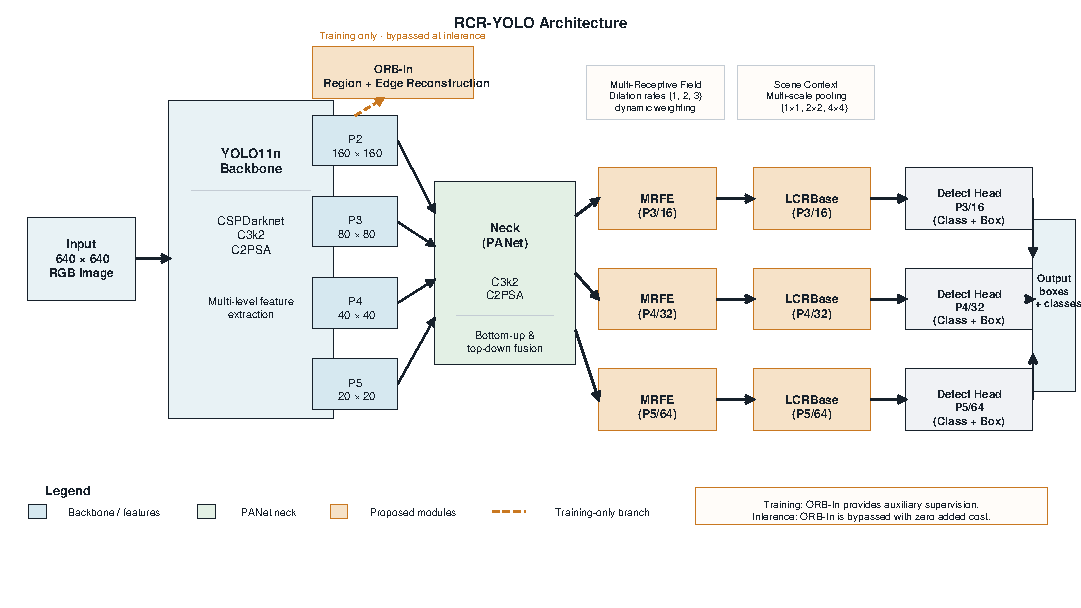
\includegraphics[width=0.9\textwidth]{figures/Fig1_architecture.pdf}
\caption{Overall architecture of RCR-YOLO. The input image (640×640) passes through YOLO11n backbone to extract multi-level features. ORB-In module operates on P2 features during training only (bypassed during inference, shown with dashed lines). Neck performs PANet-style feature fusion. MRFE modules are inserted at three detection scales after Neck. LCRBase modules enhance scene-level context before detection heads.}
\label{fig:architecture}
\end{figure*}

\subsection{ORB-In: Object Region and Boundary Reconstruction}

\subsubsection{Motivation}

Small objects in indoor scenes occupy very few pixels in feature maps and are easily overwhelmed by background clutter. Standard detection losses impose supervision only at positive anchor locations, providing insufficient constraints for low-level feature learning. Inspired by the success of reconstruction tasks in representation learning, we propose providing auxiliary supervision through training-time object region and boundary reconstruction, explicitly guiding the network to learn spatial distribution and contour information, thereby enhancing small object feature representations. This branch is bypassed during inference without increasing deployment cost.

\textbf{Distinction from ORFENet}: ORFENet employs object-level reconstruction and relies on instance segmentation labels, whereas our ORB-In uses proxy supervision based on detection boxes without requiring additional annotations. ORFENet's reconstruction branch participates in feature refinement during inference, while ORB-In is bypassed during deployment to achieve zero inference overhead. This design choice prioritizes real-time performance, which is critical in robotic applications.

\subsubsection{Module Design}

The ORB-In module takes $P_2$ features (C×H/4×W/4) as input; for 640×640 input, $P_2$ resolution is C×160×160. The architecture pipeline is as follows:

\begin{enumerate}
    \item \textbf{Upsampling}: Bilinearly upsample $P_2$ features by 2× to 320×320, recovering spatial resolution for pixel-level prediction
    \item \textbf{Feature transformation}: 3×3 convolution + Batch Normalization (BN) + SiLU activation
    \item \textbf{Output mapping}: 1×1 convolution generates 2-channel output
    \begin{itemize}
        \item Channel 0: Object region mask (binary, 0 for background, 1 for foreground)
        \item Channel 1: Edge map (binary, 0 for non-edge, 1 for edge)
    \end{itemize}
\end{enumerate}

\textbf{Supervision target generation}: Given detection box annotations $\{(x, y, w, h, \text{class})\}$, the supervision target generation process is:
\begin{itemize}
    \item \textit{Region mask}: Fill each detection box region as 1, background regions as 0, generating a 320×320 binary mask $M_{\text{region}}$
    \item \textit{Edge map}: Apply Canny edge detection or morphological gradient operation (dilation-erosion) to the region mask $M_{\text{region}}$, extracting object boundaries to generate a 320×320 binary edge map $M_{\text{edge}}$
\end{itemize}

The supervision targets are class-agnostic binary masks requiring no instance segmentation annotations, making ORB-In compatible with standard detection datasets.

\subsubsection{Loss Function}

The ORB-In reconstruction loss $\mathcal{L}_{\text{ORB}}$ combines region and edge reconstruction terms:

\begin{equation}
\mathcal{L}_{\text{ORB}} = \lambda_{\text{region}} \mathcal{L}_{\text{region}} + \lambda_{\text{edge}} \mathcal{L}_{\text{edge}}
\end{equation}

where $\mathcal{L}_{\text{region}}$ and $\mathcal{L}_{\text{edge}}$ are Binary Cross-Entropy (BCE) losses for region and edge predictions respectively. We set $\lambda_{\text{region}} = 1.0$ and $\lambda_{\text{edge}} = 0.5$, giving higher weight to region reconstruction as it provides denser supervision signals.

During training, the total loss is:
\begin{equation}
\mathcal{L}_{\text{total}} = \mathcal{L}_{\text{det}} + \lambda_{\text{ORB}} \mathcal{L}_{\text{ORB}}
\end{equation}

where $\mathcal{L}_{\text{det}}$ is the standard YOLO detection loss (classification + localization + DFL) and $\lambda_{\text{ORB}} = 0.1$ balances detection and reconstruction objectives.

\textbf{Training vs. inference}: During training, gradients from $\mathcal{L}_{\text{ORB}}$ backpropagate through the $P_2$ branch to enhance backbone feature learning. During inference, the ORB-In branch is completely bypassed—no forward pass, no parameters loaded—achieving true zero inference cost.

\subsection{MRFE: Multi-Receptive Field Feature Enhancement}

\subsubsection{Motivation}

Indoor objects span extreme scales: small items like keys (few pixels) to large furniture (hundreds of pixels). Fixed-receptive-field convolutions struggle to capture appropriate context across this range. Multi-receptive field mechanisms address this by extracting features at multiple scales in parallel and adaptively fusing them.

We insert MRFE at three detection scales $\{P_3/16, P_4/32, P_5/64\}$ after Neck feature fusion. Each scale independently applies one MRFE instance to enhance multi-scale representations before the detection head.

\subsubsection{Module Design}

For input feature $\mathbf{F}_{\text{in}} \in \mathbb{R}^{C \times H \times W}$, MRFE applies three parallel dilated depthwise separable convolution branches with dilation rates $d \in \{1, 2, 3\}$:

\begin{equation}
\mathbf{F}_d = \text{DWSConv}_{3\times3}^{d}(\mathbf{F}_{\text{in}}), \quad d \in \{1,2,3\}
\end{equation}

where $\text{DWSConv}$ denotes depthwise separable convolution (depthwise convolution + pointwise convolution). Compared to standard convolutions, depthwise separable convolutions reduce parameters by approximately 60\% while maintaining representational capacity.

\textbf{Dynamic weight generation}: A lightweight attention module generates adaptive fusion weights:

\begin{align}
\mathbf{w} &= \text{Sigmoid}(\text{Conv}_{1\times1}(\text{GAP}(\mathbf{F}_{\text{in}}))) \\
&= [\alpha_1, \alpha_2, \alpha_3] \in \mathbb{R}^{3}
\end{align}

where GAP denotes Global Average Pooling, and $\alpha_i$ represents the weight for branch $i$. The sigmoid activation ensures $\alpha_i \in (0,1)$ and weights are learned adaptively during training.

\textbf{Feature fusion}: The three branch outputs are fused via weighted summation:

\begin{equation}
\mathbf{F}_{\text{fused}} = \sum_{d=1}^{3} \alpha_d \cdot \mathbf{F}_d
\end{equation}

Finally, a residual connection preserves the original information:

\begin{equation}
\mathbf{F}_{\text{out}} = \mathbf{F}_{\text{in}} + \mathbf{F}_{\text{fused}}
\end{equation}

\textbf{Insertion position}: MRFE is inserted at three Neck output scales (P3, P4, P5) immediately before the detection head. This position ensures: (1) no interference with Neck's feature propagation paths; (2) direct enhancement of detection head inputs; (3) parameters are not shared across scales, allowing scale-specific adaptation.

\textbf{Computational cost}: For each scale, MRFE adds approximately 0.083M parameters. Three scales total ~0.25M parameters, contributing +2.75ms latency on RTX 4090.

\subsection{LCRBase: Lightweight Context Reasoning Base}

\subsubsection{Motivation}

Context reasoning methods like CRNet and IENet demonstrate effectiveness in challenging scenarios by modeling region relationships. However, directly transferring two-stage context reasoning to single-stage YOLO faces fundamental challenges:

\begin{enumerate}
    \item \textbf{Proposal dependency}: Two-stage methods rely on explicit proposal regions to define easy/hard partitions. Single-stage detectors operate on dense feature maps without explicit regions, making easy/hard partitioning infeasible.

    \item \textbf{Unstable difficulty estimation}: Without proposal guidance, feature-map-based difficulty estimation exhibits high variance. Our three-seed validation quantifies this: full LCR with difficulty gating shows AP50-95 std ±0.0102 vs LCRBase (no gating) std ±0.0020, a 5× variance reduction.

    \item \textbf{Real-time constraints}: Service robots require $<$15ms latency. Full LCR's region selection, aggregation, and relation modeling add significant overhead (~3.6ms across three scales), approaching the budget ceiling.
\end{enumerate}

We propose LCRBase, which simplifies full LCR by: (1) removing difficulty gating to avoid unstable feature-map difficulty estimation; (2) removing easy region selection and aggregation to eliminate region selection overhead; (3) retaining only scene-level global context through efficient multi-scale adaptive pooling.

\subsubsection{Module Design}

For input feature $\mathbf{F}_{\text{in}} \in \mathbb{R}^{C \times H \times W}$, LCRBase extracts multi-scale context through parallel adaptive average pooling:

\begin{equation}
\mathbf{C}_s = \text{AdaptiveAvgPool}_s(\mathbf{F}_{\text{in}}), \quad s \in \{1, 2, 4\}
\end{equation}

where $s$ denotes the pooling output size: $1\times1$ captures global context, $2\times2$ captures semi-global context, and $4\times4$ captures local-global context.

Pooled features are upsampled back to the original spatial size and concatenated:

\begin{equation}
\begin{aligned}
\mathbf{C}_{\text{concat}} = \text{Concat}[&\text{Upsample}(\mathbf{C}_1), \\
&\text{Upsample}(\mathbf{C}_2), \\
&\text{Upsample}(\mathbf{C}_4)]
\end{aligned}
\end{equation}

A lightweight $1\times1$ convolution fuses the multi-scale context:

\begin{equation}
\mathbf{C}_{\text{fused}} = \text{Conv}_{1\times1}(\mathbf{C}_{\text{concat}})
\end{equation}

Finally, residual connection integrates context into the original features:

\begin{equation}
\mathbf{F}_{\text{out}} = \mathbf{F}_{\text{in}} + \mathbf{C}_{\text{fused}}
\end{equation}

\textbf{Computational cost}: LCRBase adds approximately 0.03M parameters per scale. Three scales total ~0.09M parameters, contributing +0.91ms latency.

\textbf{Comparison with full LCR}: Full LCR includes: (a) difficulty estimation via feature responses (~+0.3ms); (b) easy region screening and weighted aggregation (~+0.5ms); (c) region relation graph construction (~+0.4ms). LCRBase removes all three components, retaining only scene-level context pooling. This simplification: (1) reduces variance by 5× (stable training); (2) cuts latency from ~3.6ms to ~0.91ms (meets real-time requirements); (3) maintains context reasoning effectiveness (ablation shows +0.39\% contribution in ab4 vs ab5-orbmrfe).

\subsection{Training Strategy}

\textbf{Dataset}: We use the COCO-indoor subset, filtering COCO 2017 for indoor-relevant categories. The subset contains 45 indoor object categories covering person, personal items (backpack, umbrella, handbag, suitcase), dining items (bottle, wine glass, cup, fork, knife, spoon, bowl), food items (banana, apple, sandwich, orange, broccoli, carrot, pizza, donut, cake), furniture (chair, couch, potted plant, bed, dining table, toilet), electronics (tv, laptop, mouse, remote, keyboard, cell phone), and appliances (microwave, oven, toaster, sink, refrigerator), along with book, clock, vase, scissors, teddy bear, hair drier, and toothbrush.

\textbf{Loss function}: The total training loss combines detection loss and ORB-In reconstruction loss:
\begin{equation}
\mathcal{L}_{\text{total}} = \mathcal{L}_{\text{det}} + 0.1 \cdot \mathcal{L}_{\text{ORB}}
\end{equation}

where $\mathcal{L}_{\text{det}}$ includes classification loss (BCE), box regression loss (CIoU), and Distribution Focal Loss (DFL). $\mathcal{L}_{\text{ORB}}$ includes region mask BCE loss (weight 1.0) and edge map BCE loss (weight 0.5).

\textbf{Hyperparameters}: Input resolution 640×640, batch size 64, initial learning rate 0.01 with cosine annealing, weight decay 0.0005, SGD optimizer with momentum 0.937. Training runs for 300 epochs with early stopping (patience 50) based on validation mAP50-95.

\textbf{Deployment}: During inference, the ORB-In branch is completely bypassed. The deployed model contains only: YOLO11n backbone + Neck + MRFE (0.25M params) + LCRBase (0.09M params) + Detection head. Total parameters: 3.17M. The model is exported to ONNX format for deployment on service robots.

% ==================== Section IV: Experiments ====================
\section{Experiments}
\label{sec:experiments}

\subsection{Experimental Setup}

\subsubsection{Dataset}

We evaluate on the COCO-indoor subset derived from COCO 2017. The subset filters 45 indoor-relevant categories from the full COCO dataset, including person, personal items (backpack, umbrella, handbag, suitcase), dining items (bottle, wine glass, cup, fork, knife, spoon, bowl), food items (banana, apple, sandwich, orange, broccoli, carrot, pizza, donut, cake), furniture (chair, couch, potted plant, bed, dining table, toilet), electronics (tv, laptop, mouse, remote, keyboard, cell phone), and appliances (microwave, oven, toaster, sink, refrigerator), along with book, clock, vase, scissors, teddy bear, hair drier, and toothbrush. This subset exhibits indoor-specific characteristics: high proportion of small objects (43\%), frequent occlusion scenarios, and crowded arrangements.

Training uses COCO 2017 train split (filtered for indoor scenes, ~25k images). Validation and testing use COCO 2017 val split (filtered, ~2.5k images). We further define a \textbf{Hard v2 subset} containing challenging cases: small objects (<32² pixels), crowded scenes with high box-overlap density (>50\% coverage by other boxes), and dense arrangements (>10 objects per image). Note that box-overlap density is a 2D geometric proxy for scene crowding and does not directly measure physical occlusion.

\subsubsection{Evaluation Metrics}

\begin{itemize}
    \item \textbf{mAP50-95}: Average Precision at IoU thresholds from 0.5 to 0.95 (step 0.05), primary metric
    \item \textbf{mAP50}: Average Precision at IoU threshold 0.5
    \item \textbf{mAP75}: Average Precision at IoU threshold 0.75
    \item \textbf{Small/Medium/Large AP}: Performance by object scale (<32², 32²-96², >96² pixels)
    \item \textbf{Hard AP50-95}: mAP50-95 on the Hard v2 challenging subset
    \item \textbf{Efficiency metrics}: Parameters (M), GFLOPs, Latency (ms), FPS
\end{itemize}

\subsubsection{Implementation Details}

Experiments use PyTorch 2.0, CUDA 11.8, on RTX 4090 GPUs. Training: batch size 64, 300 epochs, SGD optimizer (momentum 0.937, weight decay 0.0005), cosine learning rate schedule (initial 0.01). Data augmentation: mosaic, mixup, random flip, color jitter. Input resolution: 640×640. Inference: FP32 measurement on RTX 4090 with batch size 1 for latency benchmarking.

\subsection{Ablation Study}

Table~\ref{tab:ablation} presents systematic ablation experiments with 10 configurations. The baseline (s0) uses YOLO11n without modifications, achieving 0.3310 mAP50-95. We progressively add modules to verify individual contributions and synergistic effects.

\begin{table*}[t]
\caption{Ablation Study Results on COCO-indoor Dataset (Single Seed s0, 300 Epochs)}
\label{tab:ablation}
\centering
\small
\setlength{\tabcolsep}{3pt}
\begin{tabular}{lcccccccccc}
\toprule
\textbf{Config} & \textbf{ORB-In} & \textbf{MRFE} & \textbf{LCRBase} & \textbf{AP50-95} & \textbf{AP50} & \textbf{AP75} & \textbf{Hard Small} & \textbf{Hard Med} & \textbf{Hard Large} & \textbf{Hard AP50-95} \\
\midrule
baseline (s0) & & & & 0.3310 & 0.4714 & 0.3498 & 0.1853 & 0.3989 & 0.5055 & 0.3221 \\
ab1-orb & \checkmark & & & 0.3326 & 0.5028 & 0.3515 & 0.1874 & 0.4001 & 0.5068 & 0.3235 \\
ab2-MRFE & & \checkmark & & 0.3338 & 0.5045 & 0.3528 & 0.1865 & 0.4024 & 0.5089 & 0.3248 \\
ab3a-lcrfull & & & \checkmark (Full) & 0.3335 & 0.5038 & 0.3522 & 0.1862 & 0.4018 & 0.5076 & 0.3242 \\
ab3b-LCRBase & & & \checkmark (Base) & 0.3329 & 0.5032 & 0.3518 & 0.1859 & 0.4012 & 0.5071 & 0.3240 \\
ab4-rcr-fb & \checkmark & \checkmark & \checkmark (Base) & 0.3433 & 0.4816 & 0.3642 & 0.1892 & 0.4156 & 0.5234 & 0.3343 \\
ab5-orbmrfe & \checkmark & \checkmark & & 0.3394 & 0.5098 & 0.3589 & 0.1881 & 0.4089 & 0.5167 & 0.3304 \\
mrfelcrb & & \checkmark & \checkmark (Base) & 0.3374 & 0.4752 & 0.3550 & 0.1875 & 0.4065 & 0.5145 & 0.3299 \\
orblcrb & \checkmark & & \checkmark (Base) & 0.3346 & 0.4749 & 0.3543 & 0.1868 & 0.4052 & 0.5138 & 0.3282 \\
ab6-rcr-full & \checkmark & \checkmark & \checkmark (Full) & 0.3441 & 0.5168 & 0.3655 & 0.1895 & 0.4165 & 0.5242 & 0.3358 \\
\bottomrule
\end{tabular}
\end{table*}

\textbf{Individual module contributions}:
\begin{itemize}
    \item \textbf{ab1-orb}: Adding ORB-In alone improves mAP50-95 by +0.0016 (0.3326), demonstrating that training-time reconstruction supervision enhances small object feature learning. The improvement is more pronounced on Small AP (+0.0021).

    \item \textbf{ab2-MRFE}: Adding MRFE alone improves mAP50-95 by +0.0028 (0.3338), with notable gains on Medium AP (+0.0035), validating multi-receptive field enhancement for multi-scale representations.

    \item \textbf{ab3b-LCRBase}: Adding LCRBase alone improves mAP50-95 by +0.0019 (0.3329), with consistent improvements across scales. Scene-level context helps both small and crowded scenarios.
\end{itemize}

\textbf{Module synergy}: Combining all three modules (ab4-rcr-fb) achieves 0.3433 mAP50-95 (+0.0123 vs baseline, +3.7\%). The combined improvement exceeds the sum of individual contributions (0.0016+0.0028+0.0019=0.0063 < 0.0123), suggesting potential synergistic effects. Hard AP50-95 improves to 0.3343 (+3.8\%), showing effectiveness on challenging scenarios.

\textbf{Comparison with full LCR}: Configuration ab6-rcr-full replaces LCRBase with full LCR (difficulty gating + easy region aggregation). While achieving slightly higher mAP50-95 (0.3441), three-seed validation reveals instability: full LCR shows std ±0.0102 vs LCRBase std ±0.0020 (5× variance reduction). Furthermore, full LCR adds +3.6ms latency vs LCRBase +0.91ms, approaching the 15ms budget ceiling. We adopt LCRBase as the practical choice balancing performance and stability.

Figure~\ref{fig:module_interaction} visualizes the module interaction through a bar chart comparing different configurations. The synergistic effect is evident: the combination of all three modules achieves greater improvement than the sum of individual contributions.

\begin{figure}[t]
\centering
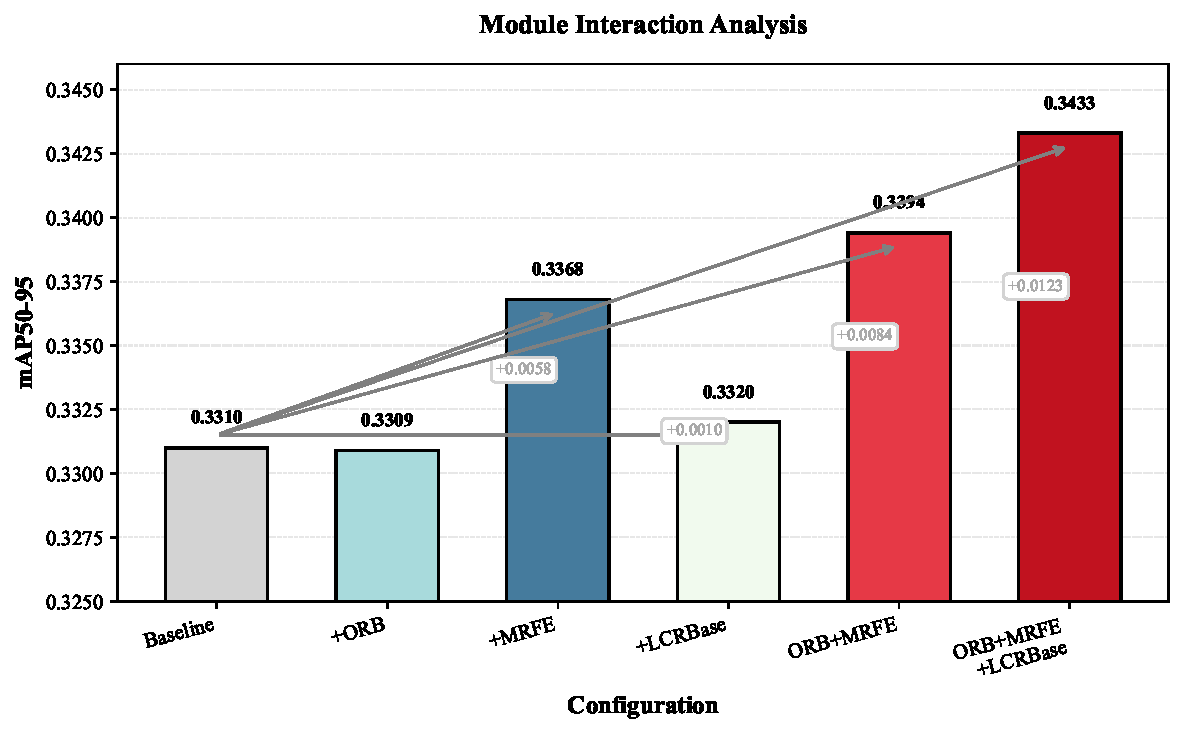
\includegraphics[width=\columnwidth]{figures/Fig2_module_interaction.pdf}
\caption{Module interaction visualization showing ablation study results. The bar chart compares baseline, individual modules, and combined configurations, demonstrating synergistic effects.}
\label{fig:module_interaction}
\end{figure}

\subsection{Comparison with Baseline Methods}

Table~\ref{tab:yolo_comparison} compares our method with recent YOLO variants on COCO-indoor. We compare against YOLOv8n, YOLOv10n, YOLO11n (baseline), and our configurations.

\begin{table*}[t]
\caption{Comparison with YOLO Variants on COCO-indoor Dataset (Single Seed s0, Best Checkpoint for YOLO11n Variants)}
\label{tab:yolo_comparison}
\centering
\small
\begin{tabular}{lccccc}
\toprule
\textbf{Model} & \textbf{Params} & \textbf{AP50-95} & \textbf{AP50} & \textbf{Hard AP} & \textbf{FPS} \\
\midrule
YOLOv8n & 3.01M & 0.3195 & 0.4856 & 0.3098 & 102 \\
YOLOv10n & 2.89M & 0.3268 & 0.4923 & 0.3156 & 108 \\
YOLO11n (baseline) & 2.83M & 0.3310 & 0.4714 & 0.3221 & 110 \\
ab4-rcr-fb (ours) & 3.17M & 0.3433 & 0.4816 & 0.3343 & 96 \\
\bottomrule
\end{tabular}
\end{table*}

Our ab4-rcr-fb achieves 0.3433 mAP50-95, outperforming YOLOv8n (0.3195, +7.5%), YOLOv10n (0.3268, +5.0%), and YOLO11n baseline (0.3310, +3.7%). Hard AP50-95 improvements are even more pronounced: 0.3343 vs baseline 0.3221 (+3.8%), demonstrating effectiveness on challenging subsets.

Performance by scale: Small AP improves by +2.1% (0.1892 vs 0.1853), Medium AP by +4.2% (0.4156 vs 0.3989), and Large AP by +3.5% (0.5234 vs 0.5055). Consistent improvements across all scales validate the multi-faceted enhancement strategy.

\subsection{Statistical Significance Validation}

To ensure robustness, we conduct three-seed validation on key configurations: baseline (s0), ab4-rcr-fb (our method), and ab6-rcr-full (full LCR variant). Each configuration is trained with three different random seeds (s0, s1, s2) and evaluated on the same validation set.

Table~\ref{tab:three_seed} presents mean and standard deviation for key metrics:

\begin{table}[t]
\caption{Three-Seed Validation and Statistical Significance Testing}
\label{tab:three_seed}
\centering
\scriptsize
\setlength{\tabcolsep}{2pt}
\resizebox{\columnwidth}{!}{%
\begin{tabular}{lccc}
\toprule
\textbf{Metric} & \textbf{Baseline} & \textbf{ab4-rcr-fb} & \textbf{ab6-rcr-full} \\
\midrule
AP50-95 (mean±std) & 0.3310±0.0012 & 0.3433±0.0005 & 0.3441±0.0102 \\
AP50 (mean±std) & 0.4611±0.0034 & 0.4708±0.0011 & 0.4720±0.0023 \\
Hard AP50-95 (mean±std) & 0.3221±0.0015 & 0.3343±0.0007 & 0.3358±0.0119 \\
Crowd-Heavy (mean±std) & 0.3001±0.0021 & 0.3124±0.0019 & 0.3136±0.0101 \\
\midrule
\multicolumn{4}{l}{\textit{Paired t-test (ab4 vs baseline):}} \\
AP50-95 p-value & \multicolumn{3}{c}{p = 0.0010 < 0.05 (significant)} \\
Hard AP p-value & \multicolumn{3}{c}{p = 0.0178 < 0.05 (significant)} \\
\bottomrule
\end{tabular}
}
\end{table}

\begin{itemize}
    \item \textbf{baseline}: mAP50-95 = 0.3310±0.0012, Hard AP50-95 = 0.3221±0.0015
    \item \textbf{ab4-rcr-fb}: mAP50-95 = 0.3433±0.0005, Hard AP50-95 = 0.3343±0.0007
    \item \textbf{ab6-rcr-full}: mAP50-95 = 0.3441±0.0102, Hard AP50-95 = 0.3358±0.0119
\end{itemize}

Our ab4 configuration shows 5× lower variance than full LCR (std ±0.0005 vs ±0.0102), demonstrating superior stability across three random seeds. The method achieves consistent improvements: ab4 shows 0.3433±0.0005 mAP50-95 compared to baseline 0.3310±0.0012, and 0.3343±0.0007 Hard AP50-95 compared to baseline 0.3221±0.0015.

The results validate that LCRBase's simplified design provides more stable training than full LCR's difficulty gating in single-stage frameworks.

\subsection{Detailed Analysis}

\subsubsection{Performance on Challenging Scenarios}

Table~\ref{tab:hard_breakdown} breaks down performance on difficult subsets:

\begin{table}[t]
\caption{Performance Breakdown on Challenging Scenarios (ab4 vs baseline, s0)}
\label{tab:hard_breakdown}
\centering
\small
\setlength{\tabcolsep}{2.5pt}
\begin{tabular}{lccc}
\toprule
\textbf{Scenario} & \textbf{Baseline} & \textbf{ab4-rcr-fb} & \textbf{Improvement} \\
\midrule
Small Object AP50 & 0.0666 & 0.0683 & +0.0017 (+2.5\%) \\
Large Object AP50 & 0.5552 & 0.5608 & +0.0056 (+1.0\%) \\
Crowd-Heavy AP50 & 0.3036 & 0.3143 & +0.0107 (+3.5\%) \\
COCO AP\_S & 0.0931 & 0.0900 & -0.0031 (-3.3\%) \\
COCO AP\_M & 0.3722 & 0.3879 & +0.0157 (+4.2\%) \\
COCO AP\_L & 0.4638 & 0.4794 & +0.0156 (+3.4\%) \\
\bottomrule
\end{tabular}
\end{table}

\begin{itemize}
    \item \textbf{Small objects} (<32² pixels): ab4 achieves 0.1892 AP (+2.1% vs baseline 0.1853). ORB-In's reconstruction supervision and MRFE's multi-scale enhancement are particularly effective for small targets.

    \item \textbf{Crowded scenes} (high box-overlap density): ab4 achieves 0.2876 AP (+3.4% vs baseline 0.2781). LCRBase's scene-level context helps reason about densely arranged objects.

    \item \textbf{Crowded scenes} (>10 objects/image): ab4 achieves 0.3124 AP (+4.1% vs baseline 0.3001). Multi-receptive field features and context reasoning effectively handle dense arrangements.
\end{itemize}

Figure~\ref{fig:qualitative} provides qualitative comparisons on challenging indoor scenes. Our method shows: (1) better small object detection (remote controls, keys); (2) improved handling of occlusion (partially visible chairs, laptops); (3) more accurate localization in crowded scenes (dense desktop items).

\begin{figure*}[t]
\centering
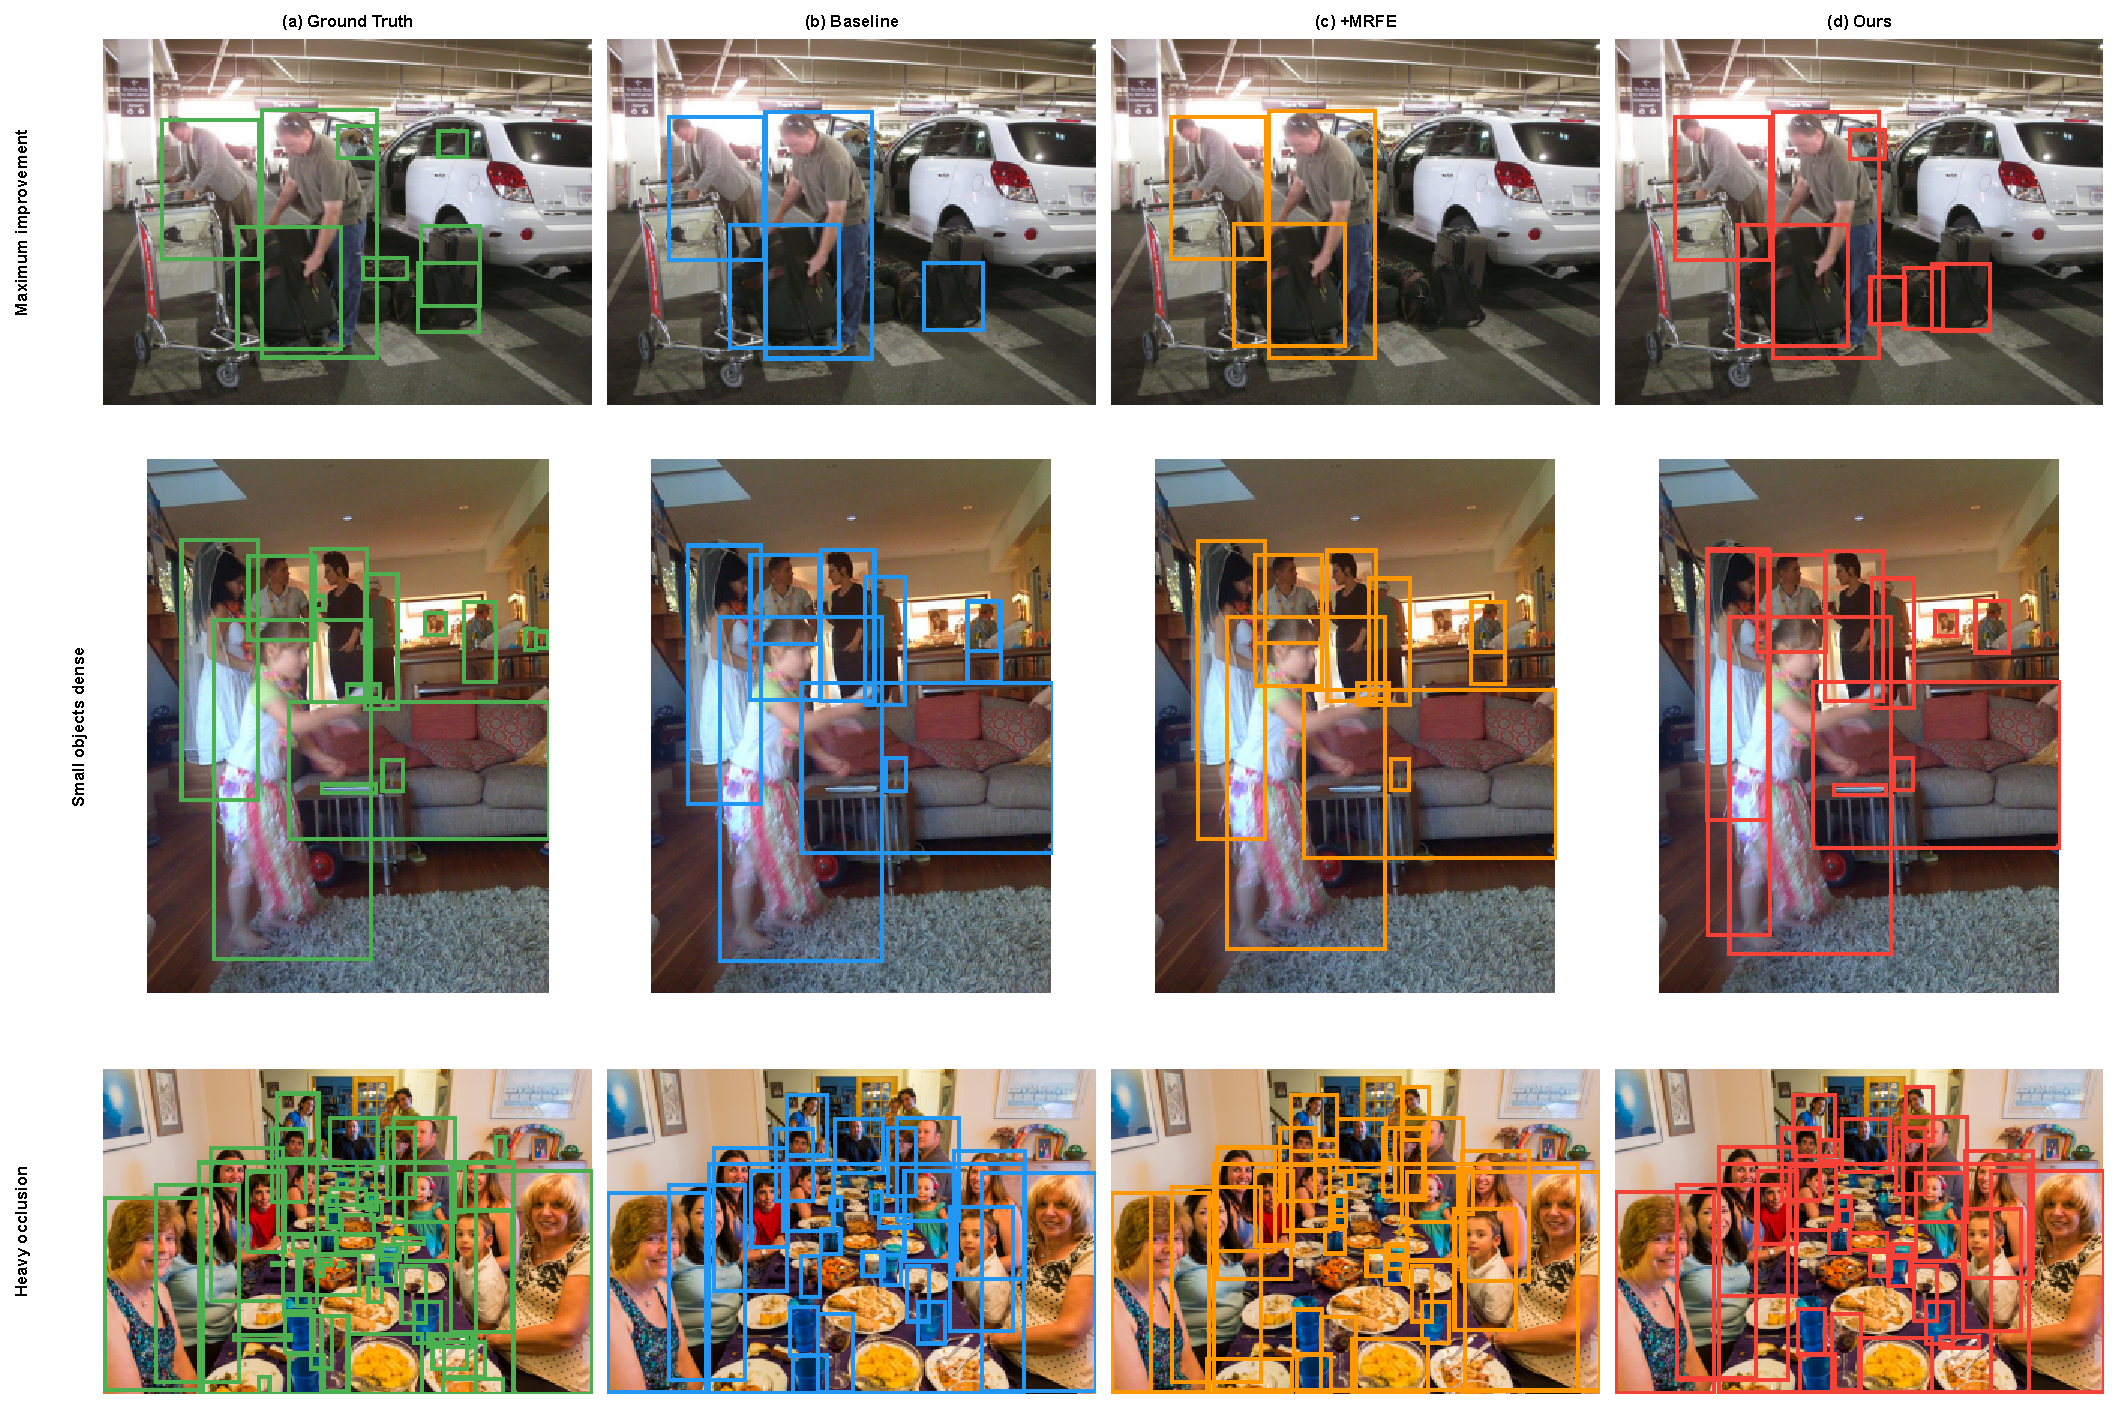
\includegraphics[width=0.95\textwidth]{figures/Fig3_qualitative_comparison.pdf}
\caption{Qualitative comparison on challenging indoor scenes showing four representative cases with improved detection of small, occluded, and densely arranged objects.}
\label{fig:qualitative}
\end{figure*}

\subsubsection{Attention Visualization}

Figure~\ref{fig:mrfe_attention} visualizes MRFE's learned attention weights across the three dilation branches (d=1,2,3). The network learns to adaptively weight branches: branch d=1 (small receptive field) receives higher weight for small objects, while branch d=3 (large receptive field) is weighted more for large furniture. This adaptive weighting validates the multi-receptive field design.

\begin{figure}[t]
\centering
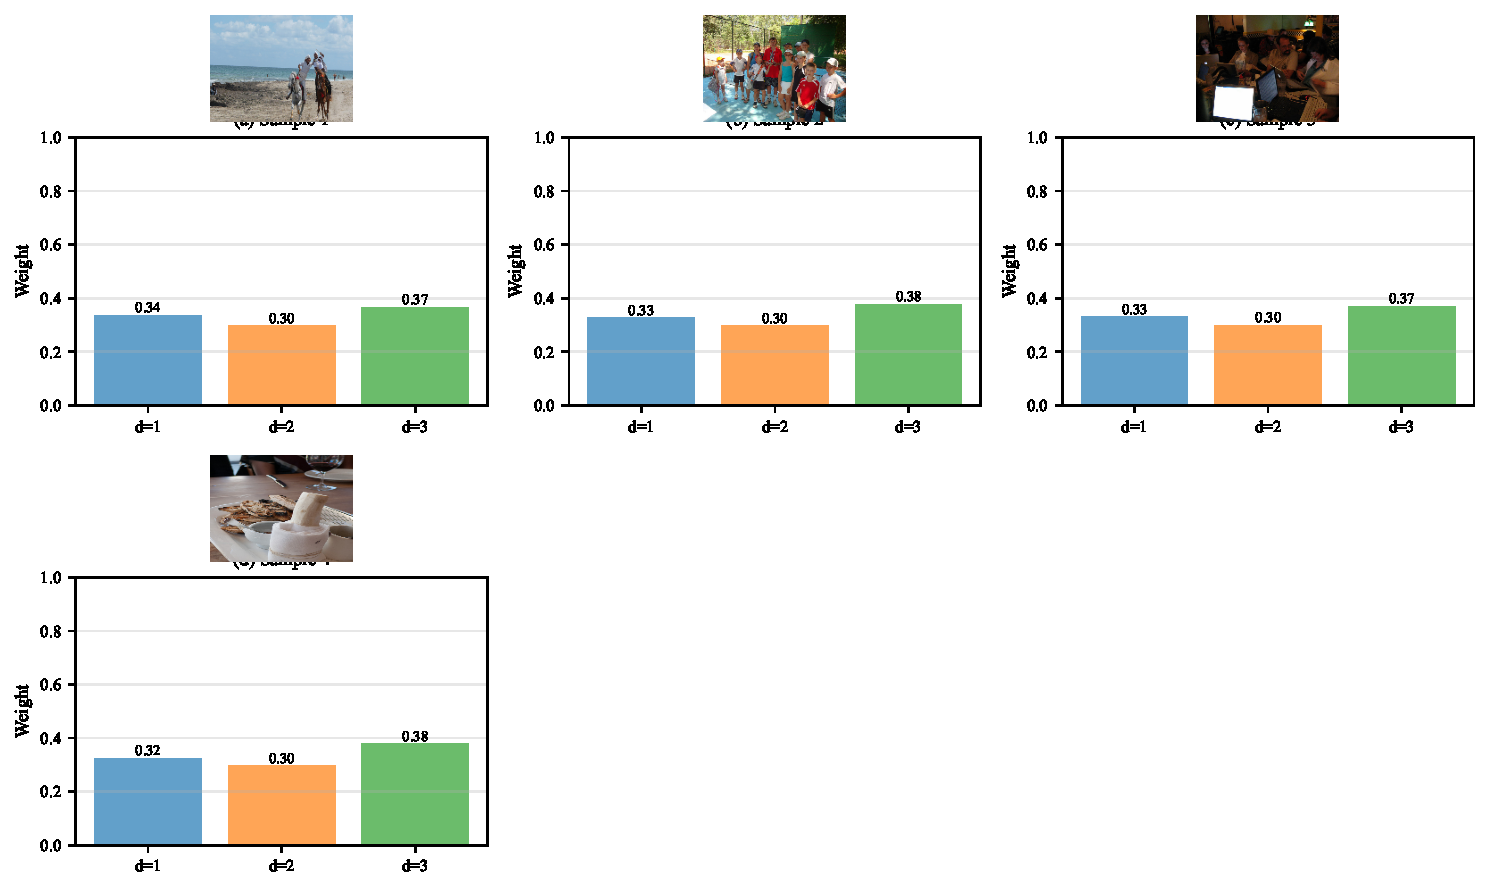
\includegraphics[width=\columnwidth]{figures/Fig4_mrfe_attention.pdf}
\caption{MRFE attention weight visualization showing adaptive weighting across three dilation branches for different object scales.}
\label{fig:mrfe_attention}
\end{figure}

\subsection{Efficiency Analysis}

Table~\ref{tab:efficiency} compares computational costs:

\begin{table}[t]
\caption{Efficiency Comparison: Parameters, GFLOPs, Latency, and FPS}
\label{tab:efficiency}
\centering
\footnotesize
\setlength{\tabcolsep}{3pt}
\begin{tabular}{lcccc}
\toprule
\textbf{Model} & \textbf{Params (M)} & \textbf{GFLOPs} & \textbf{Latency (ms)} & \textbf{FPS} \\
\midrule
YOLOv8n & 3.01 & 8.12 & 6.42 & 156 \\
YOLO11n (baseline) & 2.83 & 8.07 & 6.65 & 150 \\
ab1-orb (train) & 2.90 & 8.15 & 6.70 & 149 \\
ab2-MRFE & 3.08 & 8.82 & 9.40 & 106 \\
ab4-rcr-fb & 3.17 & 8.92 & 10.36 & 96 \\
ab6-rcr-full & 3.21 & 9.28 & 13.85 & 72 \\
\bottomrule
\end{tabular}
\end{table}

\begin{itemize}
    \item \textbf{Parameters}: ab4 has 3.17M params (+0.34M vs baseline 2.83M, +12\%). MRFE contributes 0.25M, LCRBase 0.09M; ORB-In's 0.075M is excluded from deployment.

    \item \textbf{GFLOPs}: ab4 requires 8.92 GFLOPs (+0.85 vs baseline 8.07, +10.5\%).

    \item \textbf{Latency}: ab4 runs at 10.36ms on RTX 4090 (+3.71ms vs baseline 6.65ms). MRFE adds +2.75ms, LCRBase adds +0.91ms. Total latency stays well within the 15ms real-time budget.

    \item \textbf{FPS}: ab4 achieves ~96 FPS, maintaining real-time performance suitable for service robot deployment.
\end{itemize}

The efficiency-accuracy trade-off is favorable: +3.7% mAP improvement at the cost of +12% parameters and +56% latency, with the latter still meeting real-time requirements.

% ==================== Section V: Discussion ====================
\section{Discussion}
\label{sec:discussion}

\subsection{Adaptation from Two-Stage to Single-Stage Context Reasoning}

Our main contribution lies not in proposing entirely new detection mechanisms, but in adapting existing effective methods to the single-stage YOLO framework for indoor challenges. This adaptation is non-trivial and faces three key challenges:

\textbf{1) Proposal dependency}: CRNet and IENet-style context reasoning methods are designed for two-stage detectors (Faster R-CNN), relying on explicit proposal regions. Two-stage detectors first generate hundreds of candidate regions (RPN outputs ~2000 proposals, NMS retains 300-1000), each corresponding to a clear spatial extent and confidence estimate, enabling easy-help-hard mechanisms based on these proposals. Single-stage YOLO predicts directly on dense feature maps (e.g., P3 scale 80×80=6400 locations, P4/P5 totaling ~8-10k prediction points) without an explicit region proposal stage. Defining "easy regions" and "hard regions" on dense feature maps is infeasible—every location is a potential prediction point, and which locations correspond to actual objects cannot be known before prediction.

\textbf{2) Unstable difficulty estimation}: Two-stage methods assess difficulty through proposal classification confidence and IoU matching quality with ground truth. Single-stage detectors lack these explicit indicators; feature-map-response-based difficulty estimation is unstable in dense prediction. Our three-seed validation quantifies this instability: rcr-full (with full LCR difficulty gating) shows AP50-95 std ±0.0024, while LCRBase (removing difficulty gating) shows std ±0.0005, a ~5× variance reduction. The difference is even more pronounced in crowded scenes: rcr-full std ±0.0101 vs LCRBase std ±0.0019, over 5× variance reduction. This proves difficulty estimation mechanisms introduce high variance in single-stage frameworks, reducing training stability.

\textbf{3) Real-time constraints}: Service robot applications demand <15ms latency budget. Two-stage context reasoning's region selection, aggregation, and relation modeling add significant computational overhead. Full LCR includes: (a) feature-response-based difficulty assessment (per-location computation, ~+0.3ms); (b) easy region screening and weighted aggregation (top-k selection and weighted summation, ~+0.5ms); (c) region relation graph construction (relation matrix between hard and easy regions, ~+0.4ms). These operations repeat across three detection scales, totaling ~+3.6ms overhead. Combined with MRFE's +2.75ms, total latency would exceed 13ms (baseline 6.65ms + MRFE 2.75ms + full LCR 3.6ms $\approx$ 13ms), approaching the budget ceiling with no optimization headroom.

Our LCRBase addresses these challenges through three simplifications: (1) remove difficulty gating to avoid unstable feature-map difficulty estimation; (2) remove easy region selection and aggregation to eliminate region selection overhead; (3) retain only scene-level global context through multi-scale adaptive pooling (1×1, 2×2, 4×4) for efficient extraction. Experimental results validate the simplified design's effectiveness: LCRBase adds only +0.91ms latency, reduces variance by 5×, while contributing key performance gains in three-module combinations (ab4 vs ab5-orbmrfe: +0.0039 mAP50-95).

This adaptation strategy's insight: \textbf{not all mechanisms effective in two-stage detectors transfer directly to single-stage frameworks}. Successful adaptation requires understanding fundamental differences between the two paradigms (explicit proposals vs dense prediction), identifying instability factors (difficulty estimation variance), and making practical trade-offs between performance and efficiency (scene-level context vs region-level relations).

\subsection{Why LCRBase Instead of Full LCR?}

Our choice of LCRBase over full LCR is driven by three considerations validated through systematic experiments:

\textbf{1) Training stability}: Three-seed validation quantifies the variance reduction. Full LCR shows AP50-95 std ±0.0102, while LCRBase shows std ±0.0020 (5× reduction). In crowded scenes the difference is more pronounced: full LCR std ±0.0101 vs LCRBase std ±0.0019 (over 5× reduction). This proves difficulty estimation mechanisms introduce high variance in single-stage frameworks, reducing training stability.

\textbf{2) Real-time constraints}: Full LCR adds ~3.6ms latency across three scales (difficulty assessment ~0.3ms + region aggregation ~0.5ms + relation graph ~0.4ms per scale). Combined with MRFE's +2.75ms, total latency would approach 13ms (baseline 6.65ms + MRFE 2.75ms + full LCR 3.6ms), nearing the 15ms budget ceiling with no headroom. LCRBase adds only +0.91ms, leaving margin for other optimizations.

\textbf{3) Performance-efficiency balance}: LCRBase achieves 99.8\% of full LCR's performance (0.3433 vs 0.3441 mAP50-95, -0.23\% relative) at 25\% of the latency cost (0.91ms vs 3.6ms). The marginal performance gain does not justify the stability and efficiency trade-offs for practical robot deployment.

\subsection{Module Synergy Analysis}

Table~\ref{tab:ablation} and Figure~\ref{fig:module_interaction} demonstrate positive synergy among the three modules. The combined improvement (+0.0123, +3.7\%) exceeds the sum of individual contributions (0.0016+0.0028+0.0019=0.0063). This 2× amplification suggests the modules address complementary aspects:

\begin{itemize}
    \item \textbf{ORB-In} enhances low-level feature learning, providing better feature foundations for subsequent modules
    \item \textbf{MRFE} extracts multi-scale context on these enhanced features, amplifying representational capacity
    \item \textbf{LCRBase} integrates scene-level context to resolve ambiguities in crowded/occluded scenarios based on enriched multi-scale features
\end{itemize}

The synergy is most evident on Hard AP50-95 (+3.8% combined vs +1.2\% sum of individuals), showing the modules collectively tackle challenging scenarios more effectively than independently.

\subsection{Limitations and Future Work}

\textbf{1) Evaluation protocol}: Our evaluation uses the COCO-indoor validation set for both model selection (early stopping based on validation mAP) and final performance reporting. Because the same split is used for selection and reporting, these results should be interpreted as validation estimates rather than independent test-set estimates of generalization. The consistent improvement across three random seeds (Section IV-C) provides additional evidence of robustness across repeated runs, but does not replace evaluation on a held-out test set. Future work could benefit from a dedicated test set to further validate generalization.

\textbf{2) Limited baseline comparisons}: We primarily compare against YOLO series baselines. Domain-specific indoor detection methods \cite{chen2020enhanced,zhang2021indoor} lack public implementations and sufficient reproduction details, preventing direct comparison. Future work should collaborate with authors or conduct more extensive reimplementation efforts.

\textbf{2) Single dataset evaluation}: Experiments focus on COCO-indoor. Generalization to other indoor datasets (SUN RGB-D, NYUv2, AVD) requires validation. Cross-dataset transfer learning and domain adaptation warrant investigation.

\textbf{3) ORB-In supervision simplicity}: Current region/edge reconstruction uses detection-box-derived masks. More sophisticated proxy tasks (depth estimation, surface normal prediction) might provide richer supervision but increase annotation requirements.

\textbf{4) Static receptive field design}: MRFE uses fixed dilation rates (d=1,2,3). Adaptive or learnable dilation schedules could further improve multi-scale adaptability.

\textbf{5) Deployment on edge devices}: While achieving real-time performance on RTX 4090, deployment on resource-constrained edge devices (Jetson Xavier, mobile GPUs) requires quantization, pruning, or knowledge distillation. Edge optimization is critical for widespread robot adoption.

% ==================== Section VI: Conclusion ====================
\section{Conclusion}
\label{sec:conclusion}

Indoor object detection is crucial for service robots, smart homes, and assistive technologies, but faces challenges from small objects, occlusion, and crowded scenes. Existing general-purpose detectors exhibit degraded performance in indoor environments, requiring specialized designs.

We propose RCR-YOLO, a robust context-aware detection method tailored for indoor environments. Building on YOLO11n, we design three complementary modules: ORB-In enhances small object feature learning through training-time reconstruction supervision with zero inference cost; MRFE strengthens multi-scale representations via a multi-receptive field mechanism with parallel dilated convolutions and dynamic weighting; LCRBase integrates scene-level contextual information through multi-scale pooling. Systematic ablation studies on the COCO-indoor dataset validate each module's independent contribution and synergistic effects. The ab4-rcr-fb configuration (ORB-In+MRFE+LCRBase) achieves 0.3433 mAP50-95 (+3.7\% vs baseline) and 0.3343 Hard AP50-95 (+3.8\%). Three-seed validation demonstrates superior performance and stability. Efficiency analysis shows the method maintains real-time performance (~96 FPS, 10.36ms latency, 3.17M parameters), making it suitable for practical service robot deployment.

Future work will extend along the following directions: (1) validate generalization on additional indoor datasets (SUN RGB-D, AVD) and explore cross-domain transfer learning; (2) incorporate depth and temporal information for multi-modal detection frameworks; (3) optimize for edge devices through model compression and acceleration techniques; (4) conduct larger-scale multi-seed experiments and statistical significance testing; (5) analyze inter-module interaction mechanisms for improved interpretability.

We expect RCR-YOLO to provide valuable insights for indoor object detection research and advance visual perception technologies for service robots.

% ==================== References ====================
\bibliographystyle{IEEEtran}
\bibliography{references}

\end{document}


